\documentclass[a4paper,12pt]{article}

\usepackage[utf8]{inputenc}
\usepackage[T1]{fontenc}
\usepackage{amsmath}
\usepackage{amssymb}
\usepackage{graphicx}
\usepackage{hyperref}
\usepackage{geometry}
\usepackage[italian]{babel}
\usepackage{svg}
\usepackage{float}
\usepackage{enumitem}

\geometry{a4paper, margin=1in}

\title{Progetto di Algoritmi e Protocolli per la Sicurezza}
\author{Davide D'Acunto\quad Noemi Biancamano}
\date{Gruppo 9}
\begin{document}

\maketitle

\tableofcontents
\newpage
\section{WP 1: Modello}
La seguente sezione si occupa di descrivere gli attori onesti presenti nel sistema, evidenziando le attività che sono interessati a svolgere.
\newline Successivamente, si procede alla discussione degli avversari e del threat model considerato, andando a specificare le capacità e le risorse da essi possedute. Infine, si presentano le proprietà che devono essere possedute dal sistema al fine di essere resiliente agli attacchi considerati.
\subsection{Attori \& Obiettivi}
\begin{figure}[H]
    \centering
    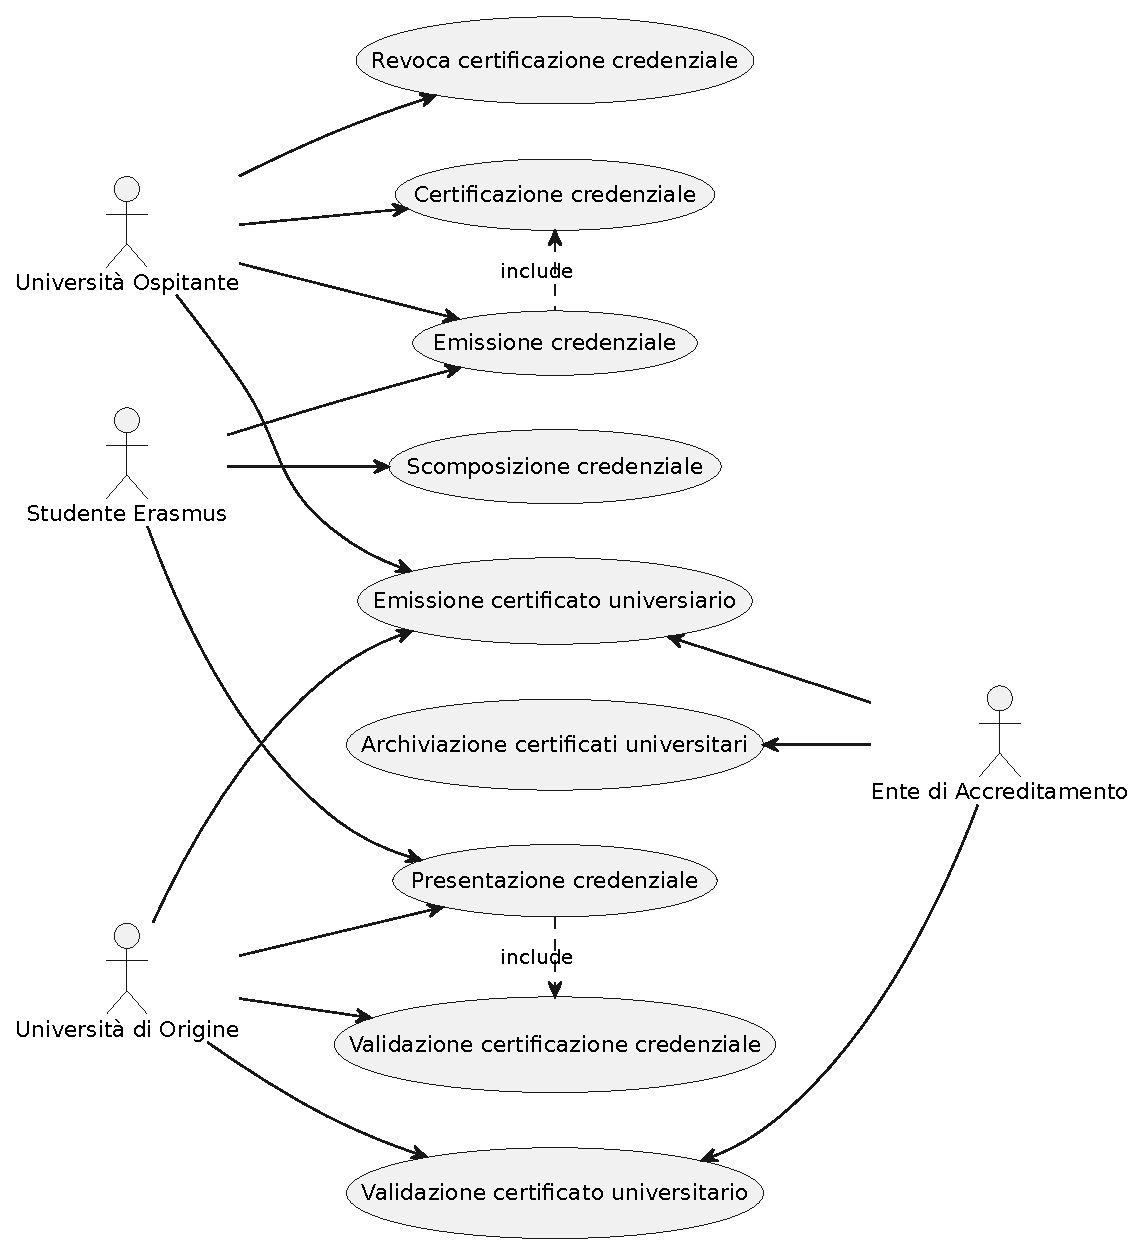
\includegraphics[width=\textwidth]{usecase_1.eps}
    \caption{Use Case degli attori onesti}
    \label{fig:usecase1}
\end{figure}
\subsubsection{Studente Erasmus}
Lo studente Erasmus è interessato a sostenere attività accademiche all'interno della sede ospitante, le quali devono essere poi certificate e dimostrate all'università di origine; per cui necessita dall'università ospitante una credenziale accademica, che attesti le attività da egli effettuate all'interno dell'università ospitante durante il periodo di mobilità. 
\newline Tale credenziale dev'essere successivamente fornita all'università di origine per certificare le attività svolte dallo studente in sede ospitante. Tuttavia, lo studente potrebbe desiderare di comunicare solamente un sottoinsieme delle informazioni contenute all'interno della credenziale, in maniera tale da dimostrare il rispetto dei criteri dell'accordo di mobilità e non rivelare informazioni personali superflue.

\subsubsection{Università Ospitante}
L'università ospitante, accordatasi con l'università di origine, permette a vari studenti erasmus di poter usufruire di un periodo di mobilità all'interno della sua sede, nel quale gli studenti hanno la possibilità di effettuare varie atttività accademiche.
\newline La sede è interessata a certificare, per ogni studente in mobilità da essa, le attività svolte da questo attraverso una credenziale, cosicché egli sia in grado di comunicarle successivamente alla sua sede d'origine.
\newline Siccome l'università ospitante non conosce i criteri definiti dall'accordo di mobilità per ciascuno degli studenti, inserisce nelle credenziali tutte le informazioni relative alle attività accademiche dallo studente, sicché sia poi in grado di poterle comunicare all'università di origine.
\newline L'ateneo inoltre desidera dimostrare che la credenziale è stata effettivamente emessa da sé, per cui richiede all'ente di accrediamento la certificazione dell'avvenuta emissione, che fornisce allo studente congiuntamente alla credenziale.
\newline Infine, in particolari casi laddove si verifichino errori amministrativi, oppure lo studente fornisca dati fraudolenti e/o cometta plagio o frode, l'università ospitante deve essere in grado di revocare la credenziale, contattando l'ente di accreditamento, cosicché da non permettere allo studente di utilizzarla.

\subsubsection{Università di Origine}
L'università di origine è accordata con l'università ospitante, mentre con lo studente attraverso un accordo di mobilità. All'interno di questo vengono definite tutte le attività accademiche che lo studente è richiesto soddisfare per validare il suo periodo di mobilità. 
\newline Per cui si aspetta di ricevere, da ciascuno studente che ha terminato il proprio periodo di mobilità, una credenziale nella quale sono presenti almeno le attività definite dall'accordo di mobilità.\newline Inoltre, la credenziale deve essere certificata da un ente di accreditamento, cosicché si abbia la certezza della validità di questa. Qualora la credenziale non fosse certificata, oppure la certificazione è invalida o revocata, l'ateneo è in grado di rifiutare la credenziale.
\subsubsection{Ente di accreditamento}
L'ente di accreditamento è un'autorità esterna, che si occupa di certificare le credenziali emesse dalle università, in modo tale da garantirne validità e autenticità. Non solo, si occupa anche dell'archiviazione delle certificazioni, conservandole sino ad una determinata data, ed eventualmente si rende disponibile ad informare gli atenei della revoca di una certificazione.\newline Infine, l'ente stabilisce, congiuntamente con le università, il formato delle credenziali, a cui gli atenei devono attenersi per essere in grado di emettere credenziali universali.
\subsection{Credenziale}
La credenziale è un documento contenente le informazioni relative alle attività accademiche che lo studente in mobilità ha svolto nella sede ospitante. 
\newline Le informazioni contenute all'interno della credenziale sono le seguenti:
\begin{itemize}
    \item Matricola interna dello studente
    \item Nome e cognome dello studente
    \item Matricola esterna dello studente
    \item Codice e nome dell'università ospitante
    \item Nome e cognome del referente dell'università ospitante
    \item Nome e cognome del referente dell'università di origine
    \item Periodo di mobilità
    \item Per ciascun esame sostenuto:
    \begin{itemize}[label=$\circ$]
        \item Nome e codice dell'esame
        \item Evebtuale voto espresso in trentesimi, oppure esito
        \item Eventuale lode
        \item CFU conseguiti
        \item Data di superamento dell'esame
        \item Nome e cognome del docente
        \item Nome e codice del corso di laurea
    \end{itemize}
    \item Per ciascuna attività svolta:
    \begin{itemize}[label=$\circ$]
        \item Nome e codice dell'attività
        \item Periodo di inizio e fine dell'attività
        \item Eventuali CFU dell'attività
        \item Nome e cognome del docente o del referente
    \end{itemize}
\end{itemize}
Le università devono attenersi a questo formato per assicurare l'interoperabilità delle credenziali emesse.
\subsection{Threat Model}
Come threat model si considerano avversari in grado di compromettere il sistema in un determinato attacco, dipendente dalle risorse e capacità da essi possedute, andando a definire quale sia la proprietà che viene meno laddove il sistema non sia resiliente a tale attacco.
\newline Ciascun attaccante viene considerato efficiente e probabilistico, ovvero con una determinata probabilità di avere successo nell'intento in tempo polinomiale.
\subsubsection{Ascoltatore tra studente e università} Si considera un attaccante in grado di ascoltare le comunicazioni che avvengono tra le università e lo studente, cercando di carpire le credenziali scambiate tra gli attori, cosicché da avere accesso a informazioni riservate dello studente.
\newline A questo punto, la proprietà compromessa è la confidenzialità delle credenziali, in quanto, sebbene possedere la credenziale di per sé non rappresenti un pericolo, l'attaccante è in grado di leggere informazioni sensibili dello studente contenute in questa.
\subsubsection{Intercettatore tra studente e università} Si considera un attaccante in grado di compromettere le comunicazioni tra gli attori, alterando le credenziali durante la loro trasmissione. L'attaccante potrebbe manipolare le informazioni contenute nelle credenziali, invalidandole o cambiando i dati in esse contenuti.
\newline In questo caso, la proprietà violata è l'integrità delle credenziali, siccome si perde la garanzia che il contenuto sia originale, ovvero che non sia stato alterato durante la trasmissione.
\newline In questo modello si aggiunge anche il caso di uno studente malevolo che tenta di fornire una credenziale alterata, non originale, o che venga impersonato dall'attaccante. In queste circostante, l'attaccante potrebbe fornire credenziali errate o alterate, per tentare di validarle.
\newline Sebbene non rappresenti una minaccia importante, vi è comunque la perdita della proprietà di autenticita dei messaggi dello studente.
\subsubsection{Intercettatore tra università e ente di accreditamento} Si considera un attaccante in grado di compromettere le comunicazioni tra l'università e l'ente di accreditamento, alterando le credenziali durante la loro trasmissione. Nel seguente caso, l'attaccante potrebbe manipolare le informazioni contenute nelle credenziali, invalidandole o cambiando i dati in esse contenuti, portando l'ente di accreditamento a rigettare il messaggio, o peggio a certificare credenziali false o alterate.
\newline La proprietà infranta è l'integrità delle credenziali, siccome si perde la garanzia che il contenuto sia originale, ovvero che non sia stato alterato durante la trasmissione.
\newline Infine, in questo modello si considera anche il caso di un attaccante che si frapponga nella comunicazione, assumento le parti dell'università dal punto di vista dell'ente di accreditamento, e viceversa. In queste circostanze, l'attaccante che assume le sembianze dell'università ospitante è in grado di:
\begin{itemize}
    \item Alterare la credenziale, per ottenere una certificazione valida di una credenziale alterata
    \item Bloccare la comunicazione, per evitare che l'università possa certificare una credenziale valida o revocare una certificazione
    \item Revocare una certificazione valida
\end{itemize}
Riguardo invece l'università di origine, l'attaccante potrebbe:
\begin{itemize}
    \item Validare una certificazione invalida
    \item Invalidare una certificazione valida
    \item Bloccare una richiesta di validazione, per evitare che l'università possa validare una credenziale
\end{itemize}
Per cui si aggiunge anche una perdita della proprietà di autenticità delle credenziali, in quanto non si ha la certezza che la credenziale sia stata emessa da un'autorità competente.

\subsection{Definizioni formali}
In questa sezione riportiamo le definizioni formali delle proprietà predentemente citate. 
\newline 
Lo schema di cifratura di riferimento utilizzato per le formalizzazione delle proprietà successive è $\Pi =\mathsf{(Gen,Enc,Dec)}$, dove: 
\begin{itemize}
    \item $\mathsf{Gen}$ è l'algoritmo di generazione di un determinato numero di chiavi, necessario alla cifratura e decifratura dei messaggi, la cui sicurezza dipende dal parametro di sicurezza $n$.
    \item $\mathsf{Enc}$ è l'algoritmo di cifratura, che produce un messaggio cifrato, detto cyphertext $c$, a partire da un messaggio in chiaro, detto plaintext $m$.
    \item $\mathsf{Dec}$ è l'algoritmo di decifratura, che produce un messaggio in chiaro, a partire da un messaggio cifrato.
\end{itemize}
Con $\mathcal{A}$ indichiamo un attaccante 

\subsubsection {Confidenzialità}
La confidenzialità è la proprietà che assicura l'accesso alle informazioni solamente a chi autorizzato. Un individuo non autorizzatto non deve essere in grado di accedere ad alcuna informazione, neanche parziale. 
\newline Si esprime la proprietà di confidenzialità tramite l'esperimento $\mathsf{Exp}_{\mathcal A,\Pi}^\mathsf{conf}(n)$,



\subsubsection {Integrità}

\subsubsection {Autenticità}

\newpage
\section{WP 2}
Describe your methodology here.
\newpage
\section{WP 3}
Describe your methodology here.
\newpage
\section{WP 4}
Describe your methodology here.


\end{document}